\documentclass[12pt,a4paper]{article}
\usepackage[slovene]{babel}
\usepackage{geometry}
\geometry{legalpaper, margin=1in}
\usepackage{graphicx}
\usepackage{soul}
\usepackage{xcolor}
\usepackage{gensymb}
\usepackage{alltt}
\usepackage{multirow}


\begin{document}

\title{Zemeljsko magnetno polje}
\author{Urh Trinko}
\maketitle

\newpage


\section{UVOD}

Pri vaji se zemeljsko magnetno polje meri s pomo\v cjo dveh metod. Prva je meritev s kompenzacijo. Pri tej meritvi postavimo tuljavo pod nekim kotom glede na smer sever-jug, ki jo dolo\v cimo s pomo\v cjo kompasa. Nato spreminjamo tok v tuljavi, dokler rezultanata sil (igla kompasa) ne ka\v ze v smeri simetrale kotov vektorjev gostote magnetnega polja tuljave in Zemlje. V tem primeru sta velikosti teh vektorjev enaki in  velja:

\begin{equation}
	{B_{Z} = B_{T} = \frac{\mu_0 N I}{\sqrt{L^{2} + (2r)^2}}} 
\end{equation}

($B_{Z/T}$ - gostota magnetnega polja Zemlje/tuljave, $N$ - \v stevilo ovojev, $I$ - tok, ki te\v ce po tuljavi, $L$ - dol\v zina tuljave, $2r$ - premer tuljave)
\\
\\
Drug na\v cin je Gaussova metoda. Pri tej je treba opraviti dve meritvi. Najprej moramo izmeriti nihajni \v cas pali\v castega magneta v zemeljskem magnetnem polju. Iz nihajne ena\v cbe pri majhnih amplitudah sledi:

\begin{equation}
	{\omega_0 = \sqrt{\frac{p B_{Z}}{J}}} 
\end{equation}

($p$ - magnetni moment pali\v castega magneta, $J = m(r^2 / 4 + h^2 / 12)$ - vztrajnostni moment valja mase $m$, vi\v sine $h$ in radija $r$ okoli navpi\v cne osi)
\\
Pri drugi meritvi pa gledamo odklon kompasove igle od osi sever-jug v odvisnosti od oddaljenosti pali\v castega magneta od kompasa. Pri tem velja naslednja relacija:

\begin{equation}
	{tan \alpha = \frac{B_{P}}{B_{Z}} = \frac{\mu_0}{4 \pi r^3} \frac{p}{B_{Z}}}
\end{equation}

Pri tem upo\v stevamo, da za gostoto magnetenega polja pali\v castega magneta, $B_{P}$ v ekvatorialni ravnini velja:

\begin{equation}
	{B_{Z} = - \frac{\mu_0 p}{4 \pi r^3}}
\end{equation}


\section{NALOGA}

\begin{enumerate}
	\item Dolo\v ci vodoravno komponento zemeljskega magnetnega polja s pomo\v cjo obeh zgoraj opisanih metod.
	\item Dolo\v ci megnetni moment pali\v castega magneta.
\end{enumerate}


\section{POTREB\v S\v CINE}

\begin{itemize}
	\item tuljava na vrtljivi letvi s pritrjenim kompasom
	\item nastavljivi tokovni izvor
	\item ampermeter, \v zice, upor 15 $\Omega$
	\item ravnilo s kompasom
	\item nihalo - vrvica s pali\v castim dr\v zalom v obliki tulca
	\item \v stoparica, tehtnica, kljunasto merilo
\end{itemize}

\section{MERITVE}

\begin{itemize}
	\item Podatki o tuljavi: L = (60.0 $\pm$ 0.2) cm, $(2r)_{L}$ = (134.18 $\pm$ 0.02) mm, $(2r)_{D}$ = (123.32 $\pm$ 0.02) mm, N = 60
	\item Podatki o pali\v castem magnetu: h = (46.38 $\pm$ 0.02) mm, $(2r)$ = (15.70 $\pm$ 0.02) mm, masa = (33 $\pm$ 1)g
	\item Podatki o tulcu: h = (49.90 $\pm$ 0.02) mm, $(2r)_{2}$ = (19.00 $\pm$ 0.02) mm, $(2r)_{1}$ = (15.78 $\pm$ 0.02) mm, masa = (6 $\pm$ 1)g
\end{itemize}

\vspace{0.5cm}

\section{IZRA\v CUNI}

\subsection{Izra\v cun zemeljskega magnetnega polja na dva na\v cina}

\subsubsection{Meritev s kompenzacijo}

Iz meritev sem dobil spodnjo tabelo:

\begin{center}
	\begin{tabular}{ |c|c| } 
		\hline
		zasuk [$\degree$] & tok [mA]\\
		\hline
		20 & 158.7 \\
		16 & 154.2 \\
		10 & 155.6 \\
		4  & 158.2 \\
		-4 & 155.1 \\
		-10& 158.9 \\
		-16& 159.3 \\
		-20& 157.2 \\  
		\hline
	\end{tabular}
\end{center}

Iz zbranih podatkov o toku sem izra\v cunal povpre\v cje in napako toka, ki je zn\v sal \hl{(157 $\pm$ 2) mA}. S pomo\v cjo tega, ena\v cbe (1) in podatkov o merilni tuljavi sem lahko izra\v cunal zemeljsko magnetno polje, ki je zan\v salo \hl{1.93 $\cdot 10^{-5}$ (1 $\pm$ 0.02) T}. Pri tem sem v ena\v cbo (1) za vrednost (2r) vstavil povpre\v cje premera na desni in levi strani tuljave.

\subsection{Gaussova metoda}

Sprva sem moral dolo\v citi nihajni \v cas pali\v castega magneta v zemeljskem magnetnem polju. \v Stirikrat izmerjen \v cas desetih nihajev je prikazan v spodnji tabeli:

\begin{center}
	\begin{tabular}{ |c| } 
		\hline
		\v cas [s]\\
		\hline
		19.607\\
		19.223\\
		19.417\\
		19.185\\  
		\hline
	\end{tabular}
\end{center}

Povpre\v cen nihajni \v cas je tako zna\v sal (1.94 $\pm$ 0.02) s. Da bi uporabil ena\v cbo (2) sem moral izra\v cunati \v se vztrajnostni moment magneta v tulcu:

$$J = J_m + J_t = m_m (r_m^2 / 4 + h_m^2 / 12) + m_t ((r^2_{t2} + r^2_{t1}) / 4 + h^2_t / 12)$$

(kjer indeks $m$ predstavlja lastnosti magneta, $t$ pa tulca)
\\
Ta vztrajnostni moment zna\v sa 7.9 (1 $\pm$ 0.06) kg$mm^{2}$. Sedaj lahko uporabim ena\v cbo (2) iz katere lahko izrazimo:

$$p B_{Z} = (\frac{2 \pi}{t_0})^2 \cdot J $$
\\
\\
Produkt  $p B_{Z}$ torej zna\v sa \hl{8.29$\cdot 10^{-5}$ (1 $\pm$ 0.08) J}(vrednost sem ozna\v cil kot A).

\newpage
Kvocient $\frac{p}{B_{Z}}$ pa lahko dobimo s pomo\v cjo ena\v cbe (3). Dane podatke sem pretvoril tako, da sem za zasuk pri dolo\v ceni oddaljenosti vzel povpre\v cje kotov, ko je bil magnet obrnjen v eno ali drugo smer. Nato sem izra\v cunal tangens teh kotov in nanesel podatke na graf tan$\varphi$(r). S pomo\v cjo scipy funkcije curvefit sem na te podatke "fital" krivuljo, ki jo dolo\v ca teoreti\v cna ena\v cba (3), kar je prikazano na sliki 1.

\begin{figure}[h]
	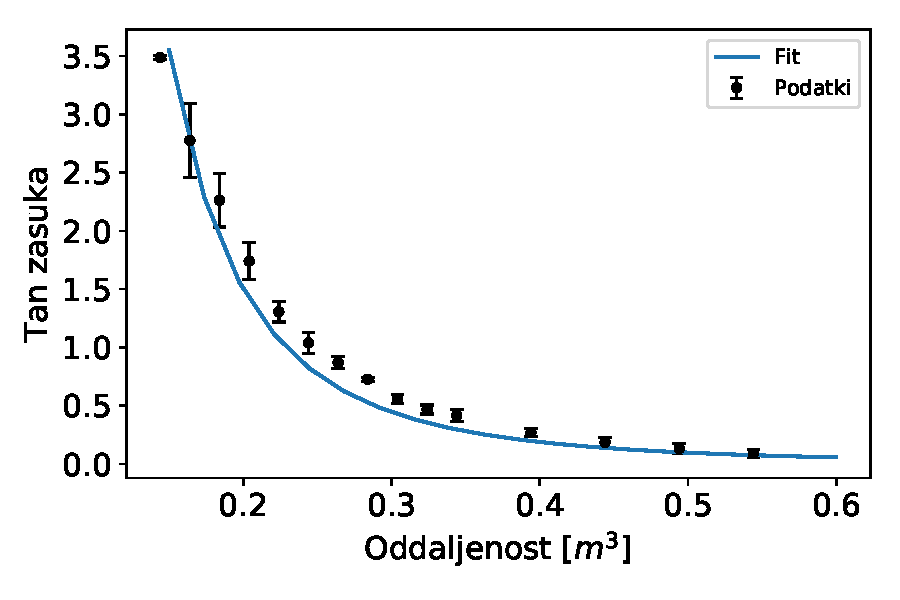
\includegraphics[width=12cm]{gauss.pdf}
	\centering
	\caption{Tangens kota zasuka igle v odvisnosti od oddaljenosti.}
\end{figure} 

S pomo\v cjo curvefit sem dolo\v ci, da je vrednost faktorja $\frac{p}{B_{Z}}$ enaka \hl{120000 (1 $\pm$ 0.18) $\frac{A m^4}{V s}$} (vrednost sem ozna\v cil kot C).
\\
S pomo\v cjo faktorjev A in C sem lahko kon\v cno dolo\v cil gostoto zemeljskega magnetnega polja preko zveze $B_{Z} = \sqrt{A / C}$. V tem primeru je vrednost zna\v sala \hl{2.6$\cdot 10^{-5}$ (1 $\pm$ 0.26) T}.

\vspace{0.5cm}

\subsection{Magnetni moment pali\v castega magneta}

Potem ko sem izra\v cunal gostoto magnetenga polja sem lahko magnetini moment pali\v castega magneta dolo\v cil iz katerekoli od dveh pridobljenih konstant (A ali B). Iz A sem lahko to vrednost dobil iz zveze $p = A / B_Z$, kar potem zna\v sa \hl{3.2 (1 $\pm$ 0.34) $A m^2$}.

\newpage

\section{ZAKLJU\v CEK IN KOMENTAR}

Pri nalogi sem na dva na\v cina izra\v cunal zemeljsko magnetno polje. Razultata pri razli\v cnih metodah sta se precej razlikovala, zato sem na interentu preveril pravo vrednost. Na\v sel sem spletno stran, na katero se lahko vnese podatke o geografski dol\v zini in \v sirini ter nadmorski vi\v sini in ti program med drugim vrne horizontalno komponento zemeljskega magnetnega polja (vir: http://wdc.kugi.kyoto-u.ac.jp/igrf/point/index.html). Ko sem vnesel podatke za Ljubljano, 46$\degree$ 3$'$ 20$''$ N, 14$\degree$ 30$'$ 30$''$ E in nadmorska vi\v sina 295 m (vir: https://en.wikipedia.org/wiki/Ljubljana), sem dobil vrednost \hl{2.21$\cdot 10^{-5}$ T}.
\\
\\
Pri ra\v cunanju me je presenetilo to, da je imel rezultat meritve s kompenzacijo bistveno manj\v so napako kot tisti, ki sem ga pridobil z Gaussovo metodo. Preden sem dobil rezultate sem bil namre\v c prepri\v can, da bo Gaussova metoda bolj natan\v cna, saj se pri metodi s kompenzacijo nana\v samo na to, da mora tisti, ki opravlja meritev oceniti, kdaj je gostota magnetnega polja v merilni tuljavi enaka Zemljini.
\\
Na koncu naloge pa sem izra\v cunal \v se magnetni moment uporabljenega pali\v castega magneta. 


















\end{document}